% !TeX spellcheck = en_US
\chapter{Model-based RL}
For many current complex situation, it's too optimistic to assume that we will know the precise model \eg, with the task of folding clothes. This section aims to learn the model.

\section{Model-based RL v.0.5}
\begin{enumerate}
	\item Run based policy $\pi_0(\textbf{a}_t| \textbf{s}_t)$ (\eg, random policy) to collect $\mathcal{D} = \{ (\textbf{s, a, s'})_i \}$
	\item Learn dynamic model $f(\textbf{s,a})$ to minimize $\sum_{i} || f(\textbf{s}_{i}, \textbf{a}_{i}) - \textbf{s}_{i}' ||^2$
	\item Plan through $f(\textbf{s,a})$ to choose actions
\end{enumerate}
\hlb{Problems:} might go beyond to new state distribution $p_{\pi_f}(\textbf{s}_t) \neq p_{\pi_0}(\textbf{s}_t)$.
\begin{itemize}
	\item If the states are discrete, we could use cross-entropy loss. If the states are continuous, we could use squared-error loss. Generally, negative log-likelihood loss.
	\item Good based policy should be taken with good care.
	\item Particularly effective \hlb{if} can hand-engineer a dynamics representation with our knowledge of physics \dots $\Rightarrow$ need to fit only a few \ac{param}
\end{itemize}

\section{Model-based RL v.1.0}
Similar solution for distribution mismatch as in \secref{subsec:dagger}.
\begin{enumerate}
	\item Run based policy $\pi_0(\textbf{a}_t, \textbf{s}_t)$ to collect $\mathcal{D} = \{ (\textbf{s, a, s'})_i \}$
	\item \tikzmark{mbrlv12}Learn dynamic model $f(\textbf{s,a})$ to minimize $\sum_{i} || f(\textbf{s}_{i}, \textbf{a}_{i}) - \textbf{s}_{i}' ||^2$
	\item Plan through $f(\textbf{s,a})$ to choose actions
	\item \tikzmark{mbrlv14}Execute these actions and \hlr{add resulting data} $\{ (\textbf{s, a, s'})_j \}$ to $\mathcal{D}$
	\begin{tikzpicture}[overlay,remember picture]
		\draw[very thick, -latex]
		([xshift=-7mm,yshift=1mm]pic cs:mbrlv14) --++ (-.5,0) |-
		([xshift=-7mm,yshift=1mm]pic cs:mbrlv12);
	\end{tikzpicture}
\end{enumerate}
\hlb{Problems:} the model would learn faster if we correct the mistake more often.

\section{Model-based RL v.1.5}
\label{sec:modelbasedrl1.5}
This is much more computational expensive compared to the above.

The more you re-plan, the less perfect each individual plan needs to be $\Rightarrow$ Can use shorter horizons. (\href{https://www.youtube.com/watch?v=LkTmiylbHYk&list=PL_iWQOsE6TfURIIhCrlt-wj9ByIVpbfGc&index=47}{YouTube}).

\begin{enumerate}
	\item Run based policy $\pi_0(\textbf{a}_t, \textbf{s}_t)$ to collect $\mathcal{D} = \{ (\textbf{\textbf{s, a, s'}})_i \}$
	\item \tikzmark{mbrlv152}Learn dynamic model $f(\textbf{s,a})$ to minimize $\sum_{i} || f(\textbf{s}_{i}, \textbf{a}_{i}) - \textbf{s}_{i}' ||^2$
	\item \tikzmark{mbrlv153}Plan through $f(\textbf{s,a})$ to choose actions 
	\item Execute the first planned action, observe resulting state $\textbf{s}' \text{ (\ac{MPC})}$
	\item \tikzmark{mbrlv155}Append $\{ (\textbf{s, a, s'})_j \}$ to $\mathcal{D}$
	\begin{tikzpicture}[overlay,remember picture]
		\draw[very thick, -latex]
		([xshift=-7mm,yshift=2mm]pic cs:mbrlv155) --++ (-.5,0) |-
		([xshift=-7mm,yshift=1mm]pic cs:mbrlv153);
		\draw[very thick, -latex]
		([xshift=-7mm,yshift=1mm]pic cs:mbrlv155) --++ (-.7,0) |-
		([xshift=-7mm,yshift=1mm]pic cs:mbrlv152);
		\node at ([xshift=-16mm,yshift=-2mm]pic cs:mbrlv153) {\fontsize{10}{0}\selectfont \rotatebox{90}{every $N$ steps}};
	\end{tikzpicture}
\end{enumerate}

\note These are all \hlb{open-loop planning}, either stochastic or deterministic, algorithms. In other words, in step 3, given a single current state, we do the planning and output a sequence of actions $\{\textbf{a}_t, \dots, \textbf{a}_{t+T}\}$. Possible planning algorithms are presented in \secref{sec:optimal-control}, \eg, random shooting, \ac{CEM}, \ac{MCTS}, \ac{LQR}.

\section{Uncertainty-aware Model}
\label{subsec:uncertainty-aware-model}
\hlb{Problem} of Model-based \ac{RL} v.1.5 (\subsecref{subsec:modelbasedrl1.5}): overfitting early, especially with high-dimensional data

\hlb{Solution:} Introduce \hlr{uncertainty estimation}\\
Step 3. Take action with \hlr{high expected reward}

This goes against exploration, thus depends on problems, use different strategies:
\begin{itemize}
	\item expected value planning
	\item optimistic value planning
	\item pessimistic value planning
\end{itemize}

\section{Uncertainty-Aware Neural Net Models}
There is two kinds of uncertainty:
\begin{itemize}
	\item \textit{aleatoric} uncertainty (statistical data uncertainty)
	\item \textit{epistemic} uncertainty (model uncertainty)
\end{itemize}
\hlr{"The model is certain about the data, but we are not certain about the model"}. Model uncertainty is then the uncertainty about \ac{param} $\theta$ that represents the model. Usually, we estimate:
\[ \underset{\theta}{\arg\max} \log p(\theta| \mathcal{D}) = \underset{\theta}{\arg\max} \log p(\mathcal{D} | \theta) \]
Or estimate the exact $p(\theta| \mathcal{D})$, then predict according to $\displaystyle \int p(\textbf{s}_{t+1} | \textbf{s}_t, \textbf{a}_t, \theta) p(\theta|\mathcal{D}) d\theta$

\begin{itemize}
	\item Use output entropy $p(\textbf{s}_{t+1} | \textbf{s}_t, \textbf{a}_t)$: predicts aleatoric uncertainty, which is the wrong one. Thus, it's \hlb{bad, not going to work}.	
	\item Bayesian neural network: \hlr{complicate} \cite{blundell2015icml}, \cite{gal2017concrete}.
	\begin{figure}[hbt!]
		\centering
		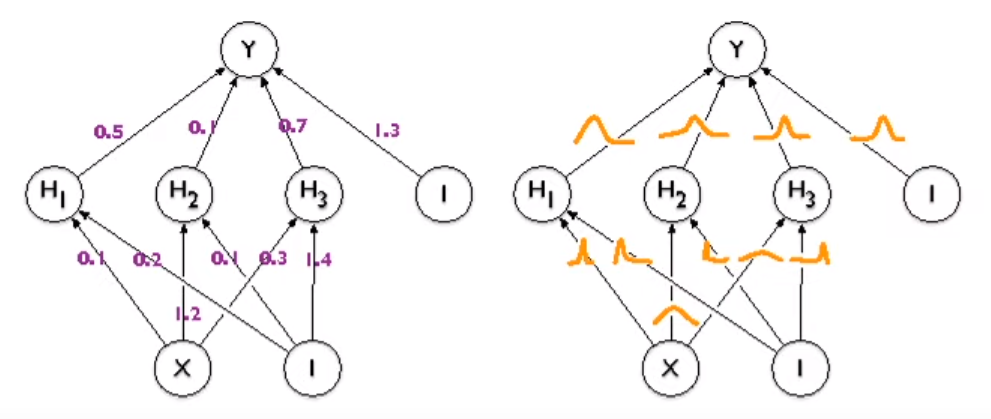
\includegraphics[width=.7\textwidth]{bayesian-neural-network.png}
		\caption{Normal neural network (left) and Bayesian neural network (right).}
	\end{figure}
	\begin{align}
		p(\theta | \mathcal{D}) & = \prod_{i} p(\theta_i | \mathcal{D}) && \text{common approximation}\\
		p(\theta_i | \mathcal{D}) & = \mathcal{N}(\mu_i, \sigma_i) && \text{common choice for each marginal \ac{prob}}
	\end{align}
	\item Bootstrap ensembles: train ensemble of models (\secref{sec:bagging}). Each model (usually $<10$ models) with \ac{param} $\theta_i$ is trained on a dataset $\mathcal{D}_i$, which is sampled with replacement from $\mathcal{D}$.
	\begin{align}
		&p(\theta | \mathcal{D}) \approx \frac{1}{N} \sum_{i} \delta(\theta_i) && \text{mixture of delta \ac{func}}\\
		&\int p(\textbf{s}_{t+1} | \textbf{s}_t, \textbf{a}_t, \theta) p(\theta|\mathcal{D}) d\theta \approx \frac{1}{N} \sum_i p(\textbf{s}_{t+1} | \textbf{s}_t, \textbf{a}_t, \theta)
	\end{align}
\end{itemize}

\section{Planning with Uncertainty}
As mentioned before, the model uncertainty is used in step 3 of the model-based \ac{RL} algorithm (\subsecref{subsec:uncertainty-aware-model}). The change is about the reward function that we use to do optimal control for action planning:
\begin{itemize}
	\item Before: $\displaystyle J(\textbf{a}_1,\dots, \textbf{a}_H) = \sum_{t=1}^{H} r(\textbf{s}_t, \textbf{a}_t)$ where $\textbf{s}_{t+1} = f(\textbf{s}_t, \textbf{a}_t) $
	\item Now: $\displaystyle J(\textbf{a}_1,\dots, \textbf{a}_H) = \frac{1}{N} \sum_{i=1}^{N} \sum_{t=1}^{H} r(\textbf{s}_{t,i}, \textbf{a}_{t,i})$ where $f(\textbf{s}_{t,i}, \textbf{a}_t) = \textbf{s}_{t+1, i}$ (deterministic case)
\end{itemize}

General procedure for candidate action sequence $\textbf{a}_1,\dots, \textbf{a}_H$:
\begin{enumerate}
	\item Sample $\theta \sim p(\theta | \mathcal{D})$
	\item At each time step $t$, sample $\textbf{s}_{t+1} \sim p(\textbf{s}_{t+1} | \textbf{s}_t, \textbf{a}_t, \theta) $
	\item Calculate $R = \sum_{t} r(\textbf{s}_t, \textbf{a}_t)$
	\item Repeat step $1\rightarrow3$ and accumulate the average reward
\end{enumerate}

\section{References}
\begin{itemize}
	\item \citeaustitle{deisenroth2011icml}
	\item \citeaustitle{chua2018deep}
	\item \citeaustitle{nagabandi2020deep}
	\item \citeaustitle{feinberg2018icml}
	\item \citeaustitle{buckman2018sample}
\end{itemize}